%Master File:lectures.tex


\lesson{Probabilistic Inference}
\vspace{-1cm}
\begin{center}
  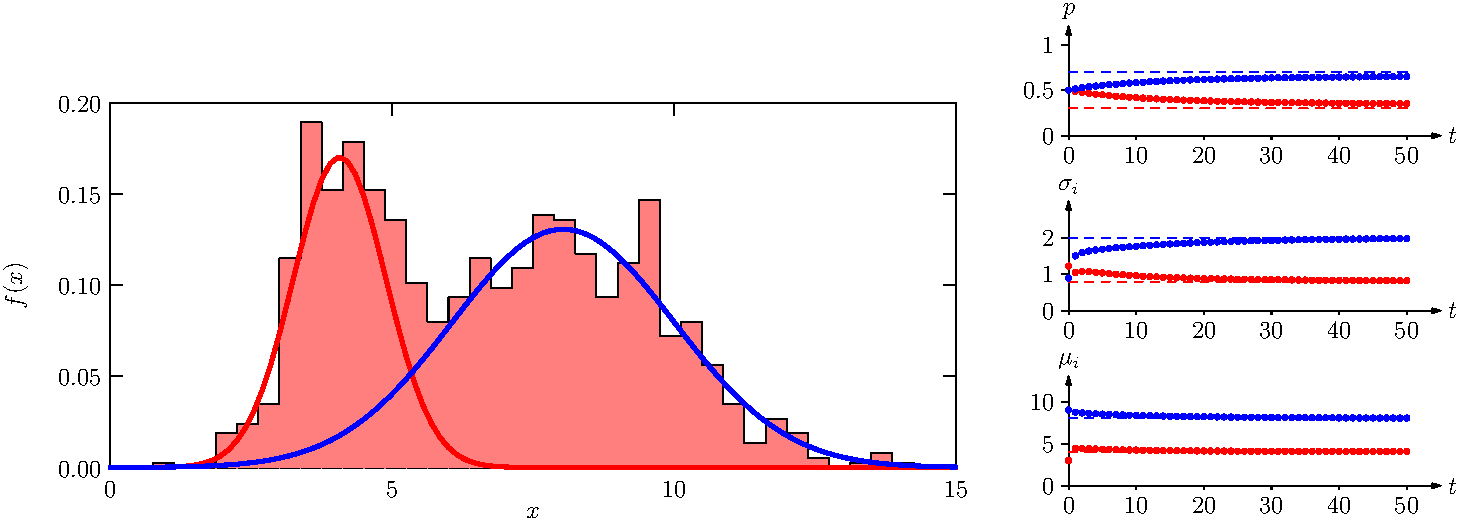
\includegraphics[width=\linewidth]{mog-1}
\end{center}
\keywords{Hierarchical Models, Mixture of Gaussians, Expectation Maximisation}
%%%%%%%%%%%%%%%%%%%%%%% Next Slide %%%%%%%%%%%%%%%%%%%%%%%
\renewcommand{\Outline}{%
\begin{slide}
\section[1]{Outline}

\begin{minipage}{10cm}\raggedright
  \begin{enumerate}\squeeze
    \outlineitem{Building Probabilistic Models}{probmodel}
    \outlineitem{Mixture of Gaussians}{mixture}
    \outlineitem{Expectation Maximisation}{em}
  \end{enumerate}
\end{minipage}\hfill
\begin{minipage}{12cm}
  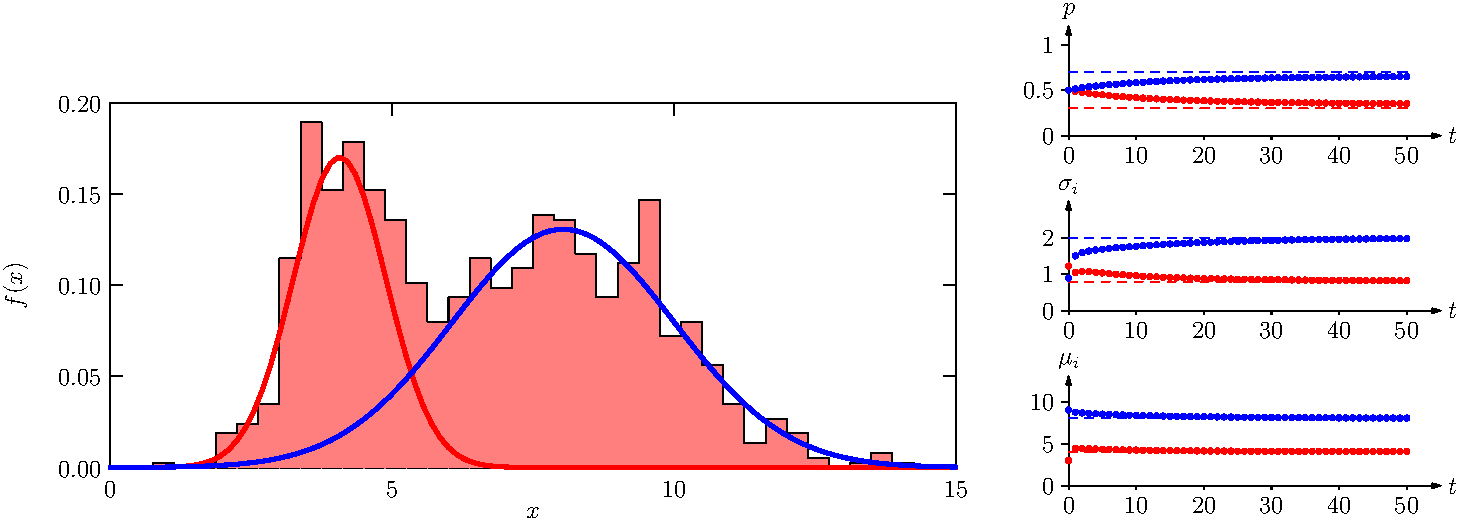
\includegraphics[width=12cm]{mog-1}
\end{minipage}
\end{slide}
\addtocounter{outlineitem}{1}
}

\setcounter{outlineitem}{1}
\Outline % Motivation
\toptarget{firstoutline}
%%%%%%%%%%%%%%%%%%%%%%% Next Slide %%%%%%%%%%%%%%%%%%%%%%%

\begin{slide}
\section[-1]{Building Probabilistic Models}

\begin{PauseHighLight}
  \begin{itemize}
  \item To describe a system with uncertainty we use random variables,
    $X$, $Y$, $Z$, etc.\pause
  \item We use the convention of writing random variables in capitals
    (this is sometimes confusing as when you observe a random variables
    it is no longer random)\pause
  \item The variables are described by probability mass function
    $\Prob{X,Y,Z}$ or if our variables are continuous, but probability
    densities $f_{X,Y,Z}(x,y,z)$\pause
  \item A major rule of probability is
    \begin{align*}
      \sum_X \Prob{X,Y,Z} &= \Prob{Y,Z}\pause
    \end{align*}
  \end{itemize}
\end{PauseHighLight}

\end{slide}

%%%%%%%%%%%%%%%%%%%%%%% Next Slide %%%%%%%%%%%%%%%%%%%%%%%

\begin{slide}
  \section{Conditional Probabilities}
  
\begin{PauseHighLight}
  \begin{itemize}
  \item When developing models it is often useful to consider
    conditional probabilities e.g.{} $\Prob{X,Y|Z}$ or
    $f_{X|Y,Z}(x|y,z)$\pause
  \item A second major rule in probabilistic modelling is
    \begin{align*}
      \Prob{X,Y} = \Prob{X|Y}\,\Prob{Y} = \Prob{Y|X}\,\Prob{X}\pause
    \end{align*}
  \item This is a mathematical identity that does not imply causality
    (it defines conditional probability)\pause
  \item It is the origins of Bayes' rule: $\Prob{X|Y} =
    \frac{\displaystyle \Prob{Y|X}\,\Prob{X}}{\displaystyle\Prob{Y}}$\pause
  \end{itemize}
\end{PauseHighLight}

\end{slide}



%%%%%%%%%%%%%%%%%%%%%%% Next Slide %%%%%%%%%%%%%%%%%%%%%%%

\begin{slide}
\section{Discriminative Models}

\begin{PauseHighLight}
  \begin{itemize}
  \item We often think of our observations as given and the predictions
    as random variables\pause
  \item For example we might be given some features $\bm{x}$ and we wish
    to predict a class $C\in\mathcal{C}$\pause
  \item Our objective is then to find the probability $\Prob{C|\bm{x}}$\pause
  \item This is known as a \emph{discriminative model}\pause
  \item E.g.{} in \textit{foundations of machine learning} you learnt how to
    find the Bayes' optimal discrimination surface\pause
  \end{itemize}
\end{PauseHighLight}

\end{slide}


%%%%%%%%%%%%%%%%%%%%%%% Next Slide %%%%%%%%%%%%%%%%%%%%%%%

\begin{slide}
\section{Generative Models}

\begin{PauseHighLight}
  \begin{itemize}
  \item Sometimes it is easy to think about the joint process of
    generating the features and outputs together\pause
  \item This leads to a joint distribution $\Prob{\bm{X},Y}$ where
    $\bm{X}$ are your features and $Y$ is your output you are trying to
    predict\pause
  \item This is known as a \emph{generative model}\pause
  \item Generative models are often more natural to think about\pause
  \item We can use them to do discrimination using
    \begin{align*}
      \Prob{Y|\bm{X}} = \frac{\Prob{\bm{X},Y}}{\Prob{\bm{X}}}
      = \frac{\Prob{\bm{X},Y}}{\sum\limits_Y \Prob{\bm{X}, Y}}\pause
    \end{align*}
  \end{itemize}
\end{PauseHighLight}

\end{slide}

%%%%%%%%%%%%%%%%%%%%%%% Next Slide %%%%%%%%%%%%%%%%%%%%%%%

\begin{slide}
\section{Latent Variables}

\begin{PauseHighLight}
  \begin{itemize}
  \item Sometimes we have models that involve random variables that we
    don't observe and we don't care about\pause
  \item These are called \emph{latent variables}\pause
  \item If we have a latent variable $Z$ and observed variable $\bm{X}$
    and we are predicting a variable $Y$ then we would
    \emph{marginalise} over the latent variable
    \begin{align*}
      \Prob{\bm{X}, Y} = \sum_Z \Prob{\bm{X}, Y, Z}\pause
    \end{align*}
  \end{itemize}
\end{PauseHighLight}

\end{slide}

%%%%%%%%%%%%%%%%%%%%%%% Next Slide %%%%%%%%%%%%%%%%%%%%%%%

\begin{slide}
\section{Modelling Virus}

\begin{PauseHighLight}
  \begin{itemize}
  \item Suppose we want to estimate the number of hospitalisation from Corona
    virus in the next month\pause
  \item Our observable is the number of reported cases\pause
  \item In our model we might want to estimate the number of actual
    cases\pause
  \item This would be a latent variable (it is not an observable or
    our final target, but it is very useful intermediate in our
    model)\pause
  \item This will be a random variable (we are uncertain, but we can
    build a probabilistic model giving a distribution of number of
    actual cases)\pause
  \end{itemize}
\end{PauseHighLight}

\end{slide}


%%%%%%%%%%%%%%%%%%%%%%% Next Slide %%%%%%%%%%%%%%%%%%%%%%%

\begin{slide}
\section{Probabilistic Inference}

\begin{PauseHighLight}
  \begin{itemize}
  \item We can use Bayes' rules to learn a set of parameter
     $\bm{\Theta}$ that occur in our likelihood function
    \begin{align*}
      \Prob{\bm{\Theta}|\mathcal{D}} =
      \frac{\Prob{\mathcal{D}|\bm{\Theta}}\, \Prob{\bm{\Theta}}}{
      \Prob{\mathcal{D}} }\pause
    \end{align*}
  \item This provides us a full probabilistic description of the
    parameters\pause
  \item It doesn't overfit (we are not choosing the best)\pause
  \item Bayesian inference provides a description of its own
    uncertainty\pause
  \item We need to specify a likelihood and prior, but this is usually
    not difficult\pause
  \end{itemize}
\end{PauseHighLight}

\end{slide}

%%%%%%%%%%%%%%%%%%%%%%% Next Slide %%%%%%%%%%%%%%%%%%%%%%%

\begin{slide}
\section{Problem with Bayes}

\begin{PauseHighLight}
  \begin{itemize}
  \item Bayes is problematic because it is often hard\pause
  \item The posterior is often not expressible as a nice probability
    function\pause 
  \item We need to compute the \textit{evidence} or \textit{margin likelihood}
    we use
    \begin{align*}
      \Prob{\mathcal{D}} = \sum_{\bm{\Theta}}
      \Prob{\mathcal{D}|\bm{\Theta}}\, \Prob{\bm{\Theta}}\pause
    \end{align*}
  \item But sometimes the number of values that $\bm{\Theta}$ can take
    are so large that we cannot easily compute this\pause
  \item Nevertheless we can usually do this using Monte Carlo techniques\pause
  \end{itemize}
\end{PauseHighLight}

\end{slide}


%%%%%%%%%%%%%%%%%%%%%%% Next Slide %%%%%%%%%%%%%%%%%%%%%%%

\begin{slide}
\section{Maximum A Posteriori (MAP) Solution}

\begin{PauseHighLight}
  \begin{itemize}
  \item One work around is to compute the mode of the posterior
    \begin{align*}
       \hspace{-1cm}\bm{\Theta}_{\text{\small MAP}} =
      \argmax_{\bm{\Theta}} \,
       f(\mathcal{D}|\bm{\Theta})\, f(\bm{\Theta})  =
       \argmax_{\bm{\Theta}} \, \logg{f(\mathcal{D}|\bm{\Theta})} +
       \logg{f(\bm{\Theta})}\pause
    \end{align*}
  \item We don't need to calculate $f(\mathcal{D})$ or explicitly
    calculate the posterior distribution\pause
  \item But it is not Bayesian (despite what you are sometime
    told)\pause---its not properly probabilistic\pauseb
  \item You can overfit and you don't get an estimate of the error in
    your inference\pause
  \end{itemize}
\end{PauseHighLight}

\end{slide}

%%%%%%%%%%%%%%%%%%%%%%% Next Slide %%%%%%%%%%%%%%%%%%%%%%%

\begin{slide}
\section{Maximum Likelihood}

\begin{PauseHighLight}
  \begin{itemize}
  \item When we assume a uniform prior then the MAP solution is just
    maximising the likelihood\pause
  \item Weirdly this hack was accepted as part of mainstream
    statistics even when Bayesian statistics was considered
    unscientific\pause
  \item Maximum likelihood is often sufficient for \textit{government
      work}, but it isn't the best you can do\pause
  \item In high-dimensional problems using a non-uniform prior
    can make a big difference\pause
  \item And, of course, doing a full probabilistic calculation has real
    advantages\pause
  \end{itemize}
\end{PauseHighLight}

\end{slide}



%%%%%%%%%%%%%%%%%%%%%%% Next Slide %%%%%%%%%%%%%%%%%%%%%%%
\Outline % Mixture of Gaussians
%%%%%%%%%%%%%%%%%%%%%%% Next Slide %%%%%%%%%%%%%%%%%%%%%%%

\begin{slide}
\section{Mixture of Gaussians}

\begin{PauseHighLight}
  \begin{itemize}
  \item Suppose we were observing the decays from two types of
    short-lived particle, $A$ or $B$\pause
  \item We observe the half life, $X_i$, but not the particle type\pause
  \item We assume $X_i$ is normally distributed with unknown means and
    variances: $\bm{\Theta} = \{\mu_A$, $\sigma_A^2$, $\mu_B$,
    $\sigma_B^2\}$\pause
  \item Let $Z_i\in\{0,1\}$ be an indicator that particle $i$ is of
    type $A$\pause
  \item The probability of $X_i$ is given by
    \begin{align*}
      f(X_i|Z_i,\bm{\Theta}) = Z_i\,\normal{X_i\big|\mu_A,\sigma_A^2} +
      (1-Z_i)\,\normal{X_i\big|\mu_B,\sigma_B^2}\pause
    \end{align*}
  \end{itemize}
\end{PauseHighLight}

\end{slide}

%%%%%%%%%%%%%%%%%%%%%%% Next Slide %%%%%%%%%%%%%%%%%%%%%%%

\begin{slide}
\section[-2]{Data}

\begin{PauseHighLight}
  \begin{itemize}
  \item Note that{\small
    \begin{align*}
      f(X_i|\bm{\Theta})
      &= \sum_{Z_i\in\{0,1\}} f(X_i,Z_i|\bm{\Theta})\pause 
        = \sum_{Z_i\in\{0,1\}}
        f(X_i|Z_i,\bm{\Theta})\,\Prob{Z_i}\pause \\
      &= \av[Z_i]{f(X_i|Z_i,\bm{\Theta})}\pause
      = p \, \normal{X_i\big|\mu_A,\sigma_A^2} +
      (1-p)\,\normal{X_i\big|\mu_B,\sigma_B^2}\pause
    \end{align*}}
  \end{itemize}
  \begin{center}
    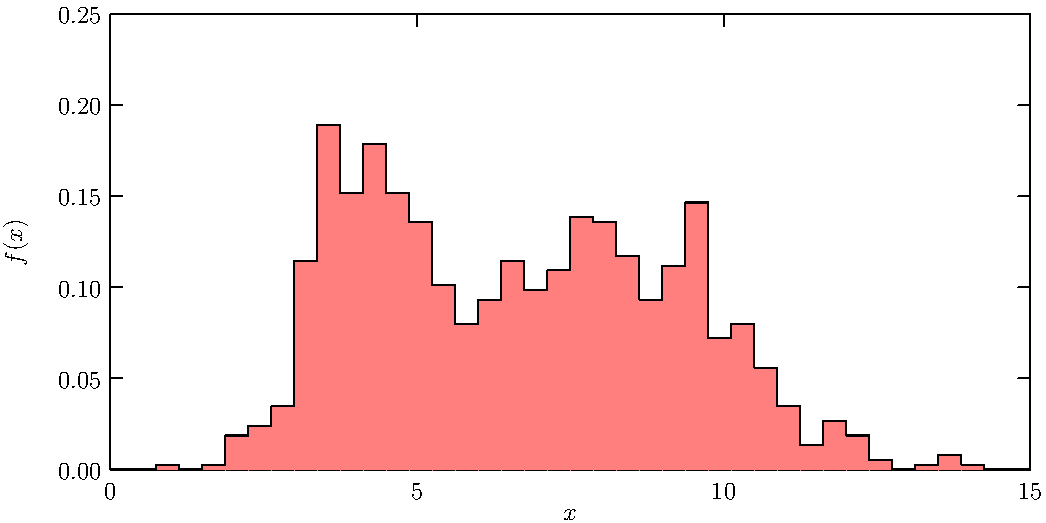
\includegraphics[width=0.8\linewidth]{mixtureOfGaussiansData}\pause
  \end{center}
\end{PauseHighLight}

\end{slide}

%%%%%%%%%%%%%%%%%%%%%%% Next Slide %%%%%%%%%%%%%%%%%%%%%%%

\begin{slide}
\section[-1]{Maximum Likelihood}

\begin{PauseHighLight}
  \begin{itemize}
  \item To solve the model as a Bayesian we would have to assign priors
    to our parameters $\bm{\Theta} = (\mu_A, \sigma_A, \mu_B,
    \sigma_B, p)$\pause
  \item This is doable, but complicated (we would also end up with a
    distribution for our parameters)\pause
  \item Often we only want a reasonable estimate for some of our
    parameters (e.g. the half-lives $\mu_A$ and $\mu_B$)\pause
  \item A reasonable approach is to seek those parameters that maximise the
    likelihood of our observed data
    \begin{align*}
      f(\data|\bm{\Theta}) = \prod_{X\in\data} f(X|\bm{\Theta})\pause
    \end{align*}
  \end{itemize}
\end{PauseHighLight}

\end{slide}


%%%%%%%%%%%%%%%%%%%%%%% Next Slide %%%%%%%%%%%%%%%%%%%%%%%
\Outline % EM
%%%%%%%%%%%%%%%%%%%%%%% Next Slide %%%%%%%%%%%%%%%%%%%%%%%

\begin{slide}
\section[-1]{Maximum Likelihood with Latent Variables}

\begin{PauseHighLight}
  \begin{itemize}
  \item The maximum likelihood is a non-linear function of the
    parameters so cannot be immediately maximised\pause
  \item If we knew which type of particle a data-point belongs to
    ($Z_i$) then it would be straightforward to maximise the
    likelihood\pause
  \item As we don't we need to estimate $\Prob{Z_i=1}$, but this
    depends on $\mu_A$, $\sigma_A^2$, $\mu_B$ and $\sigma_B^2$\pause
  \item Directly computing the maximum likelihood is a non-linear function of the
    parameters so cannot be immediately maximised\pause
  \item Although we can use a standard optimiser this is slightly inelegant\pause
  \end{itemize}
\end{PauseHighLight}

\end{slide}

%%%%%%%%%%%%%%%%%%%%%%% Next Slide %%%%%%%%%%%%%%%%%%%%%%%

\begin{slide}
\section[-1]{EM Algorithm}

\begin{PauseHighLight}
  \begin{itemize}
  \item Instead we can use an \emph{expectation-maximisation
      algorithm} usually known as an \emph{EM algorithm}\pause
  \item We proceed iteratively by maximising the expected
    log-likelihood with respect to the current set of parameters
    \begin{align*}
      \Theta^{(t+1)} = \mathop{\mathrm{argmax}}_{\bm{\Theta}}
      \sum_{\bm{Z}} \Prob{\bm{Z}\big|\data,\bm{\Theta}^{(t)}}\,
      \logg{f(\data|\bm{Z}, \bm{\Theta})}\pause
    \end{align*}
  \item It isn't obvious why this works\pause
  \end{itemize}
\end{PauseHighLight}

\end{slide}

%%%%%%%%%%%%%%%%%%%%%%% Next Slide %%%%%%%%%%%%%%%%%%%%%%%

\begin{slide}
\section{Why EM Algorithm Works}
\begin{PauseHighLight}
  \begin{itemize}
  \item The argument around why this works is quite involved\pause
  \item Note that at each step we maximise
    \begin{align*}
      Q(\bm{\Theta}|\bm{\Theta}^{(t)})
      =  \sum_{\bm{Z}\in\{0,1\}^m}
      \Prob{\bm{Z}\big|\mathcal{D},\bm{\Theta}^{(t)}}\,
        \logg{f(\mathcal{D}|\bm{Z}, \bm{\Theta})}\pause
    \end{align*}
  \item We can show that the maximum, $\bm{\Theta}^{(t+1)}$, is such
    that{\small
    \begin{align*}
      \logg{f(\mathcal{D}|\bm{\Theta}^{(t+1)})} -
      \logg{f(\mathcal{D}|\bm{\Theta}^{(t)})} \geq
      Q(\bm{\Theta^{(t+1)}}|\bm{\Theta}^{(t)}) -
      Q(\bm{\Theta^{(t)}}|\bm{\Theta}^{(t)})\pause \geq 0\pause
    \end{align*}}
  \item The details are given in the supplemental notes\pause
  \end{itemize}
\end{PauseHighLight}
  

\end{slide}

%%%%%%%%%%%%%%%%%%%%%%% Next Slide %%%%%%%%%%%%%%%%%%%%%%%

\begin{slide}
\section[-1]{Conditional Latent Variables}

\begin{PauseHighLight}
  \begin{itemize}
  \item We need to compute the distribution of latent variables
    conditioned on the data and current estimated parameters\pause
  \item For our problem
    \begin{align*}
      \Prob{\bm{Z}\big|\data,\bm{\Theta}^{(t)}} =
      \prod_{i=1}^m \Prob{Z_i\big|X_i,\bm{\Theta}^{(t)}}\pause
    \end{align*}
    where{\small
    \begin{align*}
      \Prob{Z_i=1\big|X_i,\bm{\Theta}^{(t)}} &= \frac{p^{(t)}\,
      \normal{X_i\big|\mu_A^{(t)},\sigma_A^{2(t)}} } 
     { p^{(t)}\,\normal{X_i\big|\mu_A^{(t)},\sigma_A^{2(t)}} +
     (1-p^{(t)})\, \normal{X_i\big|\mu_B^{(t)},\sigma_B^{2(t)}} } \\
      \Prob{Z_i=0\big|X_i,\bm{\Theta}^{(t)}} &= 1 -
      \Prob{Z_i=1\big|X_i,\bm{\Theta}^{(t)}}\pause
    \end{align*}}
  \end{itemize}
\end{PauseHighLight}


\end{slide}



%%%%%%%%%%%%%%%%%%%%%%% Next Slide %%%%%%%%%%%%%%%%%%%%%%%

\begin{slide}
\section{EM for Mixture of Gaussians}

\begin{PauseHighLight}
  \begin{itemize}
  \item Maximise with respect to parameters $\bm{\theta}$
    {\small
      \begin{align*}
       \hspace{-1.5cm} Q(\bm{\theta}|\bm{\theta}^{(t)})
      &=\!\! \sum_{\bm{Z}} \Prob{\bm{Z}|\data,\bm{\Theta}^{(t)}}\,
        \logg{f(\data|\bm{Z}, \bm{\Theta})} \pause
        = \sum_{i=1}^m \sum_{Z_i }\Prob{Z_i|\data,\bm{\Theta}^{(t)}}\,
        \logg{f(X_i|Z_i, \bm{\Theta})}\pause
        \\
      &=\!\!\sum_{i=1}^m \sum_{Z_i\in\{0,1\}} \Prob{Z_i|X_i,\bm{\theta}_i}\,
        \bigl( Z_i \log(p) + (1-Z_i)\log(1-p) \\
        & \hspace{9cm}  -
        \frac{(X_i-\mu_{Z_i})^2}{2\,\sigma^2_{Z_i}} - \logg{\sqrt{2\,\pi}\,\sigma_{Z_i}} \bigr)\pause
    \end{align*} }
  \item Compute update equations
    \begin{align*}
      \pd{Q(\bm{\theta}|\bm{\theta}^{(t)})}{\mu_k}=0,
      &&
         \pd{Q(\bm{\theta}|\bm{\theta}^{(t)})}{\sigma_k}=0,
      &&
          \pd{Q(\bm{\theta}|\bm{\theta}^{(t)})}{p}=0\pause
    \end{align*}
  \end{itemize}
\end{PauseHighLight}

\end{slide}

%%%%%%%%%%%%%%%%%%%%%%% Next Slide %%%%%%%%%%%%%%%%%%%%%%%

\begin{slide}
\section[-2]{Update Equations}

\begin{PauseHighLight}
  \begin{itemize}
  \item Means
    \begin{align*}
      \mu_{Z_i}^{(t+1)}
      &= \frac{ \sum_{i=1}^n \Prob{Z_i|X_i,\bm{\theta}^{(t)}} X_i}
        {\sum_{i=1}^n \Prob{Z_i|X_i,\bm{\theta}^{(t)}}},\pause
    \end{align*}
\item Variances
  \begin{align*}
    (\sigma_{Z_i}^{(t+1)})^2
      &= \frac{ \sum_{i=1}^n \Prob{Z_i|X_i,\bm{\theta}^{(t)}}
        (X_i-\mu^{(t+1)}_{Z_i})^2}
        {\sum_{i=1}^n \Prob{Z_i|X_i,\bm{\theta}^{(t)}}}\pause
  \end{align*}
  \item Probability of being type 1
    \begin{align*}
      p^{(t+1)} = \frac{1}{n} \sum_{i=1}^n \Prob{Z_i|X_i, \bm{\theta}_i}\pause
    \end{align*}
  \end{itemize}
\end{PauseHighLight}
  
\end{slide}


%%%%%%%%%%%%%%%%%%%%%%% Next Slide %%%%%%%%%%%%%%%%%%%%%%%

\begin{slide}
\section{Example}
\pause
\pb\pauselevel{=1}
\begin{center}
  \multipdf[width=\linewidth]{mixtureOfGaussians}\pause
\end{center}
\end{slide}
%%%%%%%%%%%%%%%%%%%%%%% Next Slide %%%%%%%%%%%%%%%%%%%%%%%


\begin{slide}
\section{Summary}

\begin{PauseHighLight}
  \begin{itemize}
  \item Building probabilistic models is an intricate process\pause
  \item Identifying random variables that describe the system is the
    first step\pause
  \item Often we need to introduce variables that we don't observe and
    need to be marginalised out\pause
  \item The EM algorithm provide one approach to maximising
    likelihoods or MAP solutions when we have latent variables\pause
  \item It often gives nice update equations, but convergence can be
    slow\pause
  \end{itemize}
\end{PauseHighLight}

\end{slide}


%%% Local Variables:
%%% TeX-master: "lectures"
%%% End:
